

\section{Que s'entén per Experiència d'Usuari}
Segons Rex Hartson \cite{def_UX}, l'\ac{UX} és la totalitat de l'efecte o efectes que sent (o experimenta) internament l'usuari com a resultat de la interacció, i del context d'ús, amb el sistema, dispositiu o producte. És a dir, una bona \ac{UX} es produirà quan l'usuari gaudeixi interaccionant i utilitzant el dispositiu o producte. Interacció i ús s'empren en un sentit molt ampli, ja que inclouen veure, tocar, pensar sobre el producte/dispositiu o fins i tot admirar-lo. 
A més, l'\ac{UX} també engloba la usabilitat i la utilitat. Certament l'usuari sent internament parts de la usabilitat, com l'augment de productivitat. Però hi ha certes manifestacions de usabilitat, com podria ser el temps invertit en la tasca, que representa un component no necessàriament experimentat internament per l'usuari.

\section{Com s'estudia l'\ac{UX}?}
L'\ac{UX} no pot ser dissenyada ja que depèn, no només del producte en si mateix, sinó que també depèn de l'usuari i la situació en la que l'utilitza \cite{cant_design_UX}. I és que no és possible dissenyar ni l'usuari ni la situació. Però el que si es pot fer és dissenyar per a una bona \ac{UX}. Per a aconseguir-ho hi ha quatre activitats elementals que són anàlisi, disseny, implementació i avaluació, tal i com es pot veure a la figura \ref{fig:UX_lifecycle}. Per tal d'aconseguir proporcionar una bona \ac{UX} aquestes activitats és duen a terme de forma iterativa, ja que no sempre és possible trobar un bon disseny al primer intent.

\begin{figure}[htp]
\centering
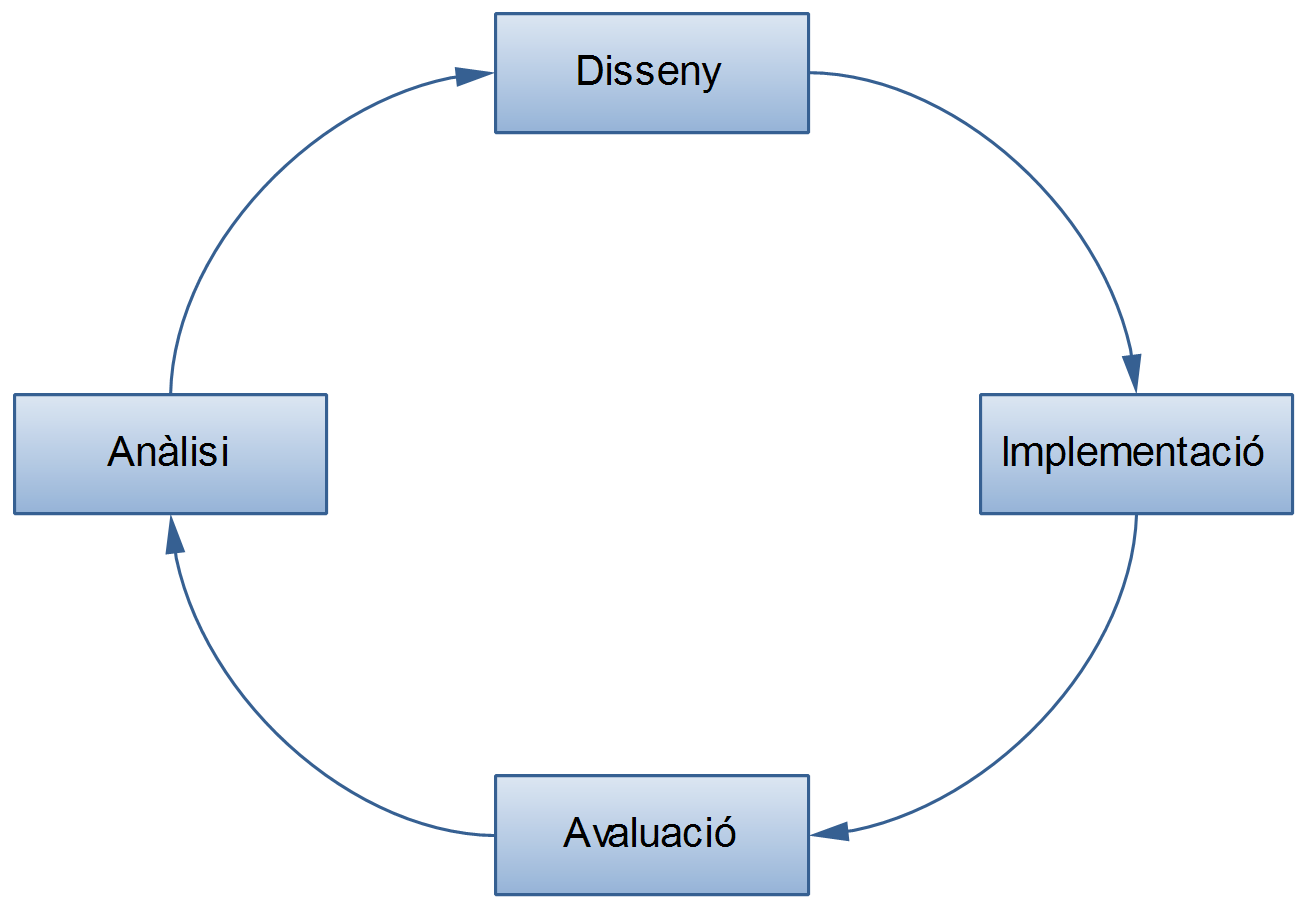
\includegraphics[scale=0.6]{UX_wheel.png}
\caption{Activitats a seguir per a dissenyar garantint una bona \ac{UX}}\label{fig:UX_lifecycle}
\end{figure}

Aquestes quatre activitats, a grans trets, consisteixen en:
\begin{description}
\item [Anàlisi] Es basa en entendre les necessitats de l'usuari que utilitzarà el producte.
\item [Disseny] Consisteix en la creació de dissenys conceptuals determinant la interacció, el comportament i l'aparença del producte.
\item [Implementació] Correspon a la creació del prototip.
\item [Avaluació] Es tracta de comprovar si el disseny satisfà les necessitats dels usuaris que s'han determinat.
\end{description}

\subsection{Anàlisi}\label{sec:analisi}
L'objectiu general d'aquesta activitat és definir com seran les usuaris potencials. Un cop definits, serviran per a poder extreure com interaccionaran amb el producte, quines necessitats tindran i en conseqüència els requeriments del producte, tal com afirma Rich Fulcher \cite{user_centred_design}.

Dins de l'anàlisi hi ha quatre subactivitats o passos a seguir:

\subsubsection{Investigació contextual}\label{subsec:investigacio_contextual}
Durant la investigació contextual s'estudia com les persones treballen o interactuen amb el producte en el seu entorn de treball. Per treball s'entén l'ús del producte en si i per entorn de treball, l'entorn en que habitualment s'usa aquest. S'utilitzen aquests termes independentment de la tipologia del producte. És a dir, encara que el producte fos un joc, al fet d'utilitzar-lo se l'anomena treballar. 

Durant la investigació contextual es tracta d'investigar i descobrir com l'usuari treballa en l'entorn habitual i això no es pot determinar enquestant als usuaris. El problema és que la descripció que pugi fer un usuari de com treballa no és fiable. La forma correcta d'investigar és observant com els usuaris treballen i entrevistant-los mentre ells duen a terme aquesta activitat. Per tant es tracta de:

\begin{itemize}
\item Preparar i realitzar visites de camp a l'entorn de treball, on el producte serà utilitzat, de l'usuari/client.
\item Observar i entrevistar els usuaris mentre treballen.
\item Indagar en l'estructura de la pròpia pràctica de treball de l'usuari.
\item Aprendre com la gent treballa en l'entorn en el qual treballarà el producte a dissenyar.
\item Extreure notes detallades de les observacions i entrevistes.
\end{itemize}

Durant la investigació contextual és important no preguntar als usuaris que volen o necessiten. En aquesta etapa no es busca que necessiten sinó observar i entrevistar els usuaris en el seu entorn de treball sobre com treballen.


\subsubsection{Anàlisi contextual}\label{subsec:analisi_contextual}
L'essència d'aquest pas és el processament, la interpretació i l'anàlisi de la informació aconseguida a la investigació contextual (apartat \ref{subsec:investigacio_contextual}). Això s'aconsegueix a base de:

\begin{itemize}
\item Crear un model de flux.
\item Sintetitzar la informació en \glspl{workActivityNotes}.
\item Construir un \ac{WAAD} a partir de les \glspl{workActivityNotes}.
\end{itemize}
%TODO Vocabulari: notes d'activitats de treball??

El model de flux és una representació gràfica que explica com les diferents entitats es comuniquen per tal d'aconseguir que el treball es realitzi. Per a poder crear el model de flux cal identificar els rols de treball. Un rol de treball és una col·lecció de responsabilitats que desenvolupen una part coherent del treball.

\begin{figure}[htp]
\centering
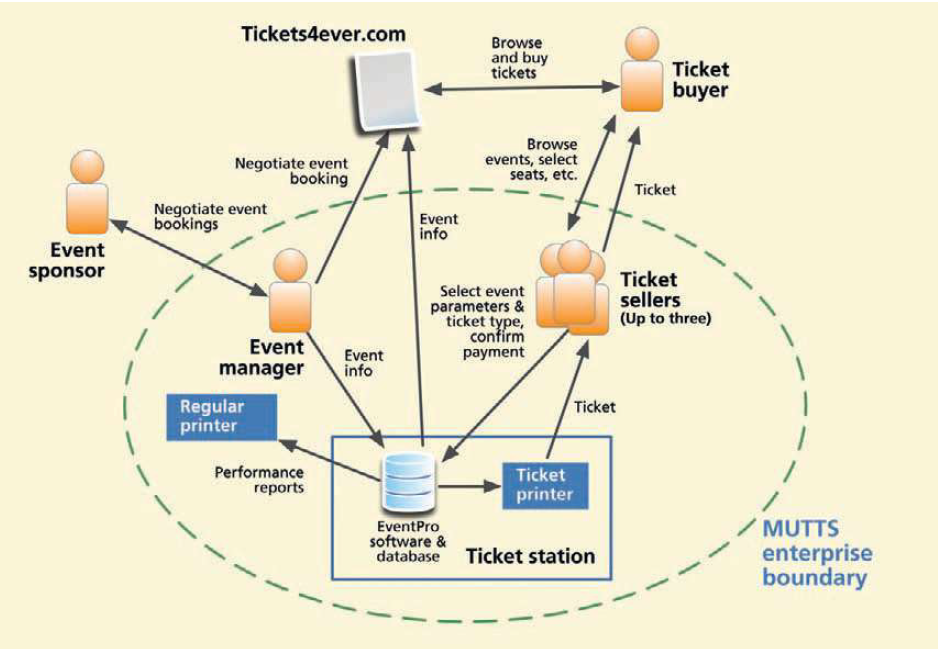
\includegraphics[scale=0.6]{flow_model_example.png}
\caption{Exemple de model de flux.}\label{fig:flow_model_example}
\end{figure}

Paral·lelament a la creació del model de flux, cal sintetitzar la informació en brut que s'ha extret a la investigació contextual. Això es fa creant \glspl{workActivityNotes} les quals, un cop tota la informació ha estat processada, han de representar tota la informació abans extreta. Aquestes notes es caracteritzen per estar escrites en primera persona (des de la perspectiva de l'usuari) parafrasejant i sintetitzant la opinió d'aquest. Cada nota ha de ser concisa i compacta, de manera que expressi una sola idea. Un exemple d'aquestes notes és el de la figura \ref{fig:workActivityNote1}. Com es pot veure cal etiquetar les notes amb un identificador representant l'usuari del qual provenen.

\begin{figure}[htp]
\centering
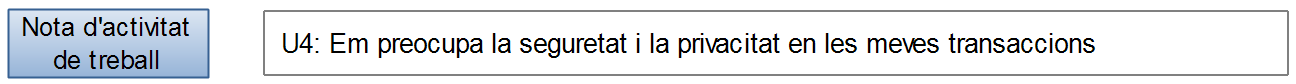
\includegraphics[scale=0.3]{WorkActivityNotes1.png}
\caption{Exemple d'una nota d'activitats de treball}\label{fig:workActivityNote1}
\end{figure}

Les \glspl{workActivityNotes} serveixen per a construir el \ac{WAAD}. Aquest diagrama consisteix en l'agrupació de les notes segons grups o afinitats segons la perspectiva de l'usuari. L'objectiu d'aquest diagrama és transmetre de forma clara i ràpida la opinió dels usuaris. El que es busca es que ja no sigui necessari llegir les llargues transcripcions de la investigació contextual ja que el \ac{WAAD} n'és una representació d'aquesta. 

%TODO Imatge representant-lo?

\subsubsection{Extracció dels requeriments d'interacció}\label{subsubsec:Extraccio_requeriments}
La idea general d'aquesta etapa es recórrer l'estructura jeràrquica del \ac{WAAD} per extreure sentencies sobre els requeriments del sistema. Això és dur a terme analitzant les \glspl{workActivityNotes} per deduir les necessitats i/o requeriments que cada nota implica. Els requeriments que s'extreuen s'han d'etiquetar per categories (i subcategories si fa falta) juntament amb un identificador que els relacioni amb la \gls{workActivityNotes} de la qual prové. Així si en un anàlisi posterior sorgeixen dubtes, es pot buscar la font de cada requeriment. 

És també important extreure aquells requeriments que l'usuari considera obvis i que per tant no menciona ni descriu i que per tant no estan implícitament a les \glspl{workActivityNotes}.

\begin{figure}[htp]
\centering
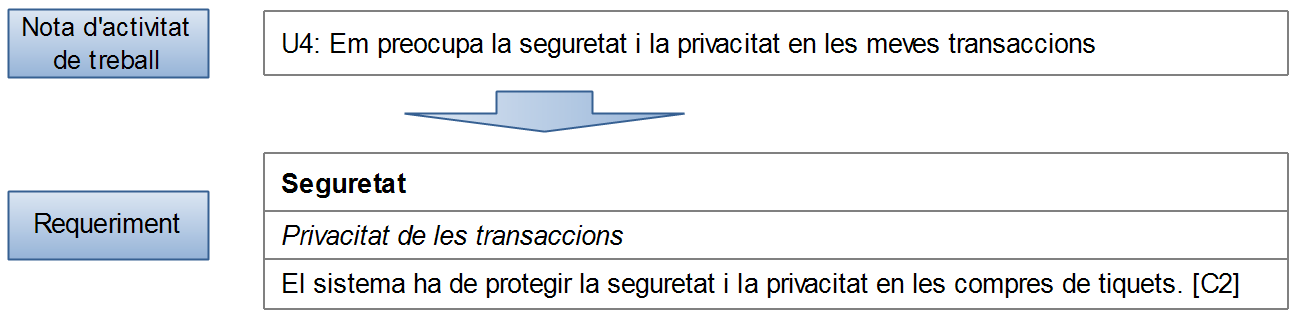
\includegraphics[scale=0.3]{WorkActivityNotes2.png}
\caption{Exemple d'extracció de requeriments}\label{fig:workActivityNote2}
\end{figure}

A la figura \ref{fig:workActivityNote2} es pot veure com s'extreu un requeriment, utilitzant el mateix exemple que abans (figura \ref{fig:workActivityNote1}). L'etiqueta "C2", fa referencia a la posició que ocupava la nota dins el \ac{WAAD}.
%TODO Especificar millor que vol dir C2.

Un cop generats els requeriments es comprovarà que aquests siguin correctes preguntant directament als usuaris. Sempre que sigui possible es preguntarà als usuaris que van participar en la investigació contextual (apartat \ref{subsec:investigacio_contextual} juntament amb d'altres nous usuaris. Aquest pas també pot servir perquè els usuaris ajudin a destacar aquells requeriments que són prioritaris.

\subsubsection{Construcció de models informatius per al disseny}
Per dur a terme aquesta etapa també cal recórrer el \ac{WAAD}, és per això que aquesta etapa no és posterior a l'etapa \ref{subsubsec:Extraccio_requeriments} sinó que les dues es duen a terme de forma paral·lela. L'objectiu d'aquesta etapa és obtenir una sèrie de documents que descriuen tant el sistema actual, com el sistema que es preveu. Aquests documents seran els que es faran servir per a dissenyar el nou producte.

%Per a facilitar la comprensió, es farà servir d'exemple l'estudi d'\ac{UX} per a crear una aplicació per a demanar pizzes, el mateix que fan servir N. Idris i I. Grey \cite{udacity_UX}.

\subsection{Disseny}

%TODO Pagina 161 - 196 5.0.0
\subsection{Implementació}
\subsection{Avaluació}